\documentclass{beamer}
%\documentclass[handout]{beamer}
\usepackage{etex}
\usepackage[utf8]{inputenc}
\usepackage[T1]{fontenc}
\usepackage[ngerman]{babel}
\usepackage{color}
\usepackage{colortbl}
\usepackage{amsmath}
\usepackage{amsfonts}
\usepackage{amssymb}
\usepackage{mathabx}
\usepackage{textcomp}
\usepackage{natbib}
\usepackage{multirow}
\usepackage{nicefrac}
\usepackage{multicol}
\usepackage{url}
\usepackage{gb4e-}
\usepackage{pifont}

\title[Topic Domains]{Automatic Classification by Topic Domain for Meta Data Generation, Web Corpus Evaluation, and Corpus Comparison}
\author[Roland Schäfer, Felix Bildhauer]{Roland Schäfer$^1$ and Felix Bildhauer$^2$}
\institute[]{$^1$Ling.\ Web Characterization (DFG), FU Berlin\\ $^2$Institut für Deutsche Sprache, Mannheim}
\date[]{10th Web as Corpus Workshop, ACL 2016, Berlin\\August 12, 2016}

\usetheme{default}
\usecolortheme{beaver}

\newcommand*\rot{\rotatebox{90}}

\begin{document}

%\titlegraphic{\includegraphics[width=0.2\textwidth]{fulogo}\hspace{0.05\textwidth}
\includegraphics[width=0.125\textwidth]{dfglogo}\hspace{0.25\textwidth}
\includegraphics[width=0.2\textwidth]{idslogo}}
%\frame{\titlepage}

\begin{frame}
%\begin{textblock*}%{2cm}(.35cm,-8cm)                                                                                          
%  \includegraphics[scale=.48]{hukombi_bwb}
\includegraphics[width=0.25\textwidth]{fulogo}\hspace{0.05\textwidth}
\includegraphics[width=0.10\textwidth]{dfglogo}\hspace{0.4
\textwidth}
\includegraphics[width=0.2\textwidth]{idslogo}
%  \end{textblock*}
  \maketitle
\end{frame}


\begin{frame}
  {Background}
  \begin{itemize}
    \item \alert{Reliable metadata}: not available for large crawled web corpora
    \item \alert{Topic domain} (and genre/register): essential for many corpus linguists
    \item Also important for \alert{corpus evaluation} and corpus comparison\\
%      \citep{Kilgarriff2001,BiemannEa2013,SchaeferBildhauer2013de}
      \vspace{0.5cm}
    \item Automatic classification by \alert{genre/register}: disappointing results, even in recent experiments.
    \item \citet{BiberEgbert2016}: acc.=0.42, prec.=0.27, rec.=0.3
  \end{itemize}
\end{frame}


\begin{frame}
  {Automatic classification by content}  
  \begin{itemize}
    \item Promising results years ago already \citep{Sebastiani2002}.
    \item \alert{Data-driven induction of topics}: a very objective way of organizing a collection of documents by content.
    \item Topic classification through internal criteria: also advocated in the \citet{EAGLES1996} guidelines
   \end{itemize}
  
  \vspace{0.5cm}     
  But:
  \begin{itemize}
    \item \alert{Topic modeling}: no category labels
    \item from a linguist's viewpoint: categories should be `intuitively' interpretable
  \end{itemize}
  \end{frame}


  \begin{frame}
    {Experiment}
    Idea
    \begin{enumerate}
      \item Infer a topic distribution over a corpus using topic modeling algorithms (\alert{unsupervised})
      \item Do not interprete the inferred topical structure directly.
      \item Instead, learn a small set of topic domains from the documents' assignment to the topics (\alert{supervised})
    \end{enumerate}
\pause
    Goals
    \begin{itemize}
      \item Development of a suitable annotation scheme for topic domain,\\
      grounded in lexical distributions
      \item Corpus comparison: web corpus vs.\ newspaper corpus\\
       (very little is known about the composition of crawled web corpora)
    \end{itemize}
    \end{frame}


\begin{frame}
  {COWCat}
  Text classification schema  \citep{SchaeferBildhauer2012a}\\

  \begin{itemize}
    \item No complex categories such as \textit{genre}, \textit{register} etc.
    \item Instead simple categories: \textit{Aim}, \textit{Mode}, \alert{\textit{Topic Domain}}
    \item Builds on previous work by \citet{Sharoff2006}
    \end{itemize}

\pause
    Topic Domain\\

    \begin{itemize}
    \item Design goal: moderate number (about 10--20) categories
    \item Basis for our classifcation experiments: 13 categories
    \item Developed in a cyclic fashion\\
    (repeated annotation processes, annotator feedback)
  \end{itemize}
\end{frame}

\begin{frame}
  {Step 1: Creating a gold standard data set}
  \begin{itemize}
    \item 870 documents from DECOW14\\
    (crawled web corpus, \citealp{SchaeferBildhauer2012a,Schaefer2015b})
    \item 886 documents from DeReKo\\
    (predominantly newpspaper texts; \citealp{KupietzEa2010})
    \item Manually annotated with COWCat categories for topic domains
      \vspace{0.5cm}
    \item {\footnotesize Annotators: Sarah Dietzfelbinger, Lea Helmers, Theresia Lehner, Kim Maser, Samuel Reichert, Luise Rißmann (FU Berlin); Monica Fürbacher (IDS Mannheim)}
  \end{itemize}
\end{frame}


\begin{frame}
  {Distribution of topic domains}
  Comparison of DeReKo and DECOW14\\[1cm]
  \begin{center}
    
\includegraphics[width=0.45\textwidth]{dereko}~
\includegraphics[width=0.45\textwidth]{cow}
  \end{center}
\end{frame}

\begin{frame}
  {Step 2: Topic modelling}

  \begin{itemize}
    \item Starting point: term-document matrix
    \item Documents: weighted assignment to topics
    \item Topics: defined by a set of weighted words
  \end{itemize}

  Our experiment:
  \begin{itemize}
    \item LSI (\citealp{LandauerDumais1994})\\
          LDA (\citealp{BleiEa2003})\\
          as implemented in \texttt{Gensim} \citep{RehurekSojka2010}% \nocite{LandauerDumais1994,LandauerDumais1997,BleiEa2003})
    \item LDA topic distributions unstable (small gold standard corpora)
    \item Incrementally add other documents from the source copora
     \vspace{.25cm}
    \item Input terms: lemma $+$ simplified POS tag (\textit{kindergarten\_nn}) 
    \item Filtering: best results with lower-cased, purely alphabetic noun lemmas, 4--30 chars long
    \end{itemize}
\end{frame}


\begin{frame}
  {Corpus comparison: distribution of (selected) LSI-topics}
  \begin{center}
    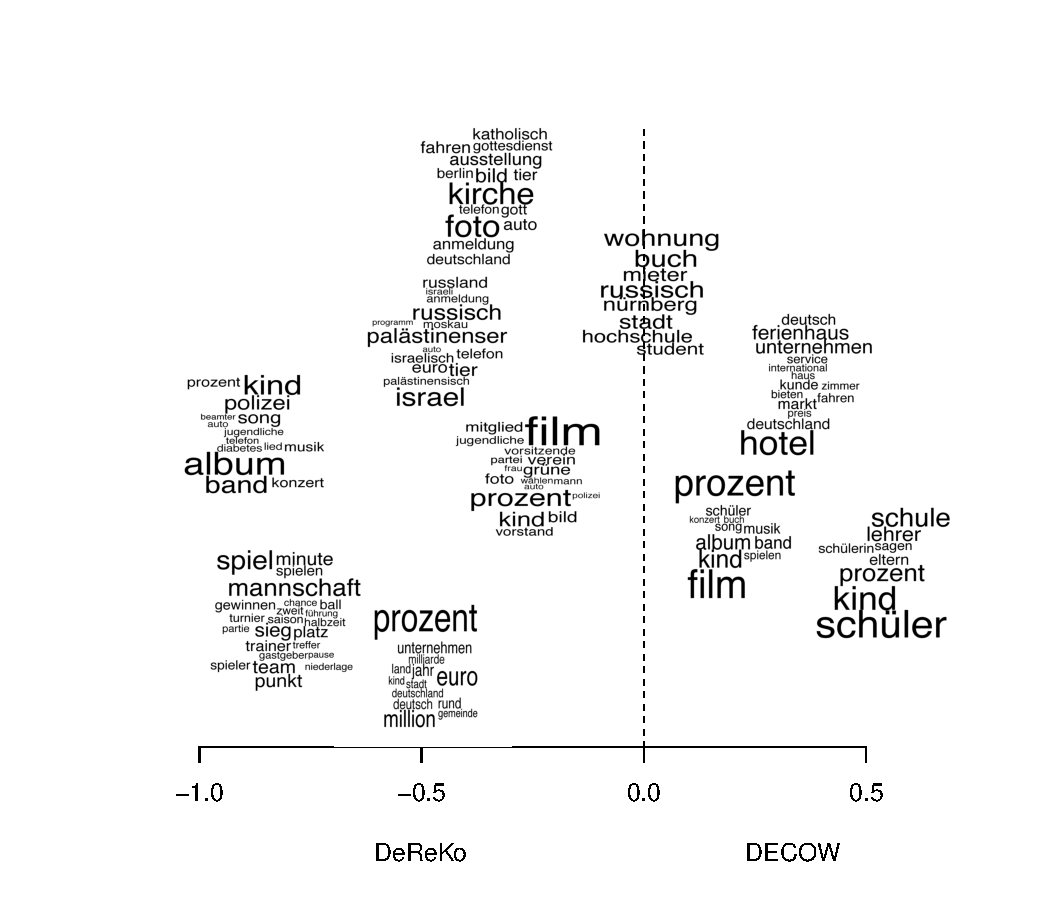
\includegraphics[width=0.75\textwidth]{topics-logratios2bw}
  \end{center}
\end{frame}




\begin{frame}
  {Step 3: Learning topic domains from LSI-topics}
  \begin{itemize}
    \item Supervised classifiers
    \item Permutation of virtually all available classifiers in \texttt{Weka}\\ \citep{HallWitten2011}
    \item Highest accuracy: SVMs with a Pearson VII kernel\\ \citep{UstunEa2006}
  \end{itemize}
  \vspace{.5cm}
\pause
Set of experiments with:
  \begin{itemize}
    \item varying number of LSI-topics
    \item topics induced from
      \begin{itemize} 
        \item gold standard data plus varying amounts of additional documents
        \item several pre-processing variants of gold standard data
      \end{itemize}
    \item evaluation on the \textit{full} data set and on a \textit{reduced} data set (with rare categories removed)
  \end{itemize}
\end{frame}

%\begin{frame}
%  {Ergebnisse}
%  COW ($\kappa$)\\
%
%  \begin{center}
%    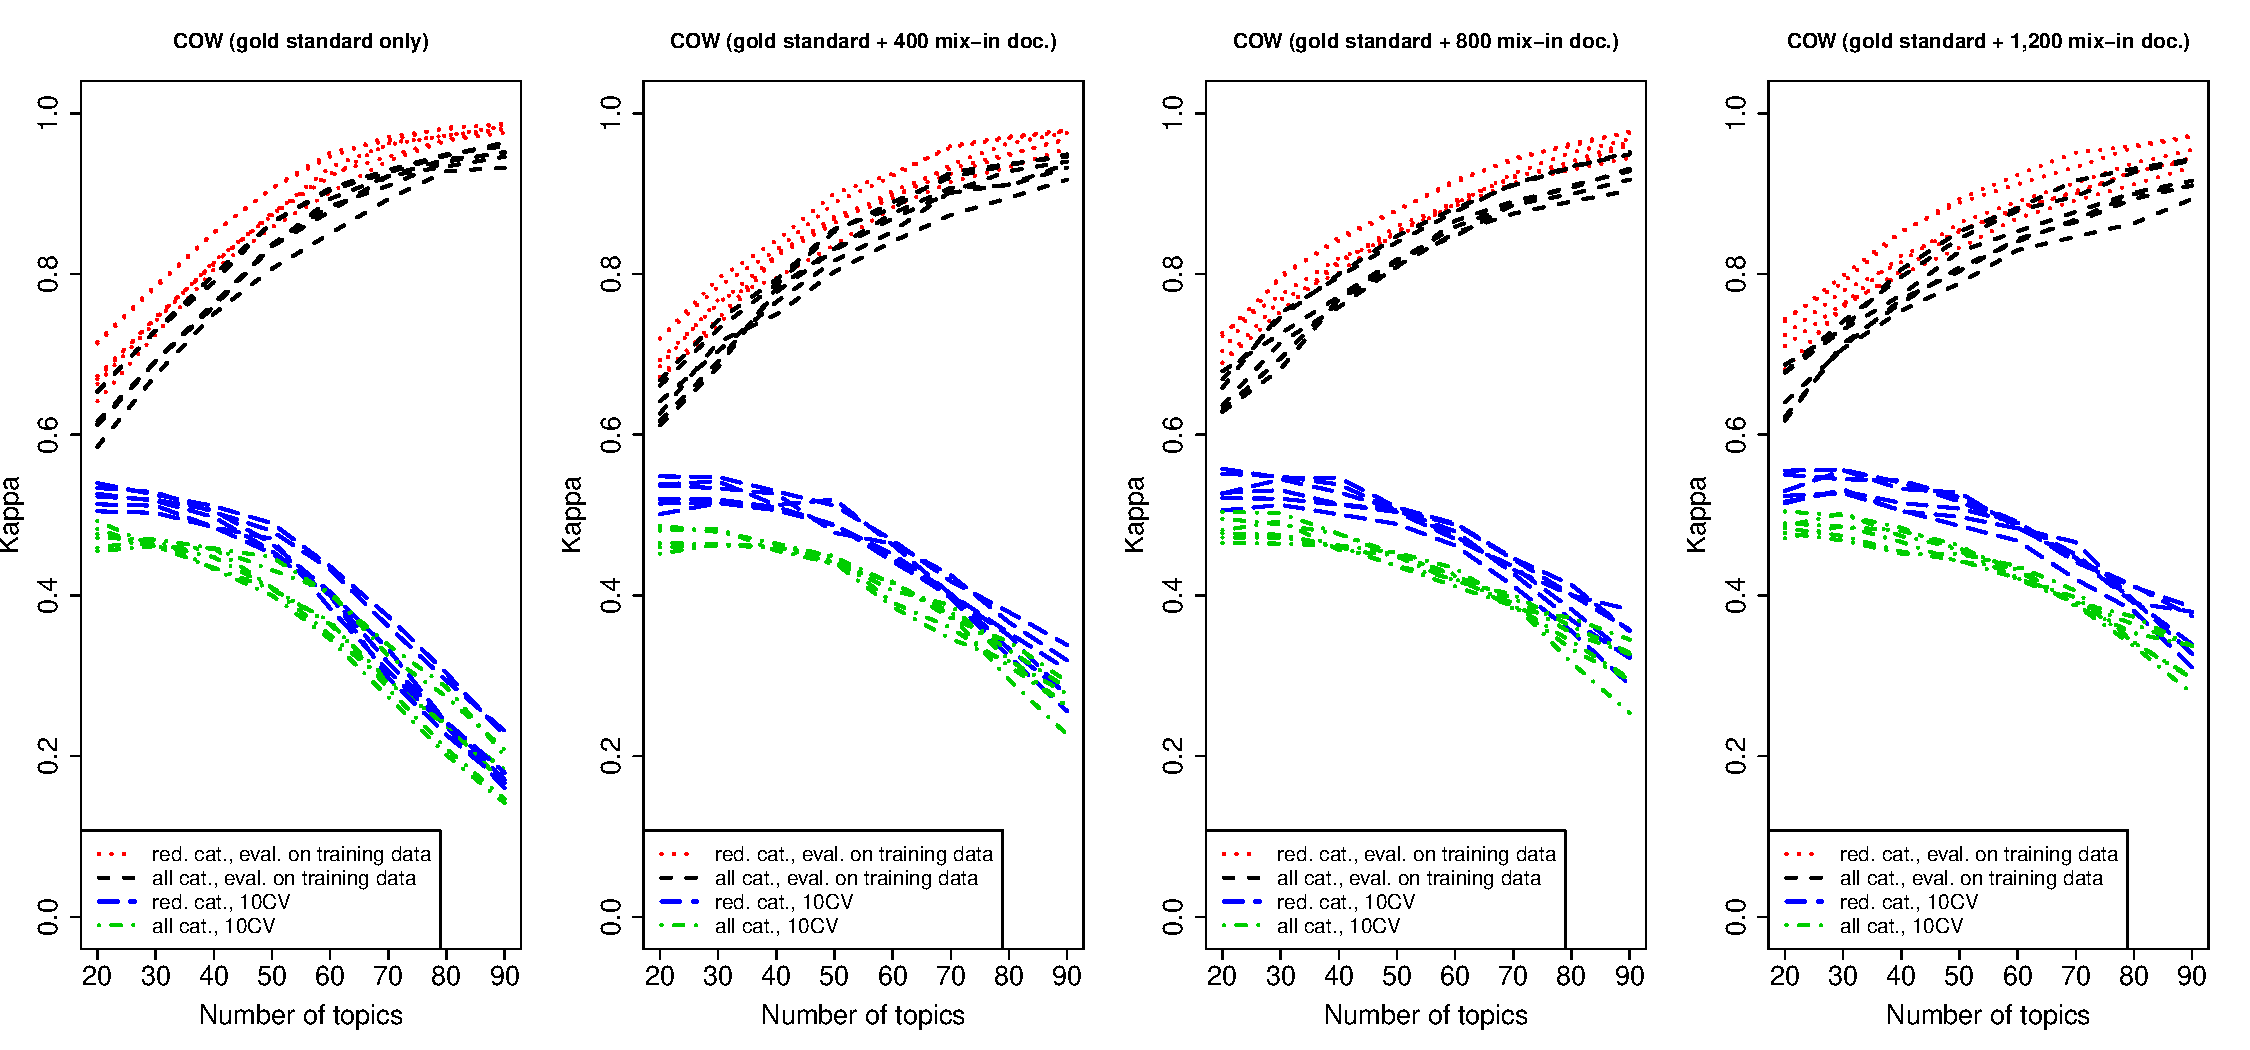
\includegraphics[width=\textwidth]{cow_kappa}
%  \end{center}
%\end{frame}
%
%\begin{frame}
%  {Ergebnisse}
%  DeReKo ($\kappa$)\\
%
%  \begin{center}
%    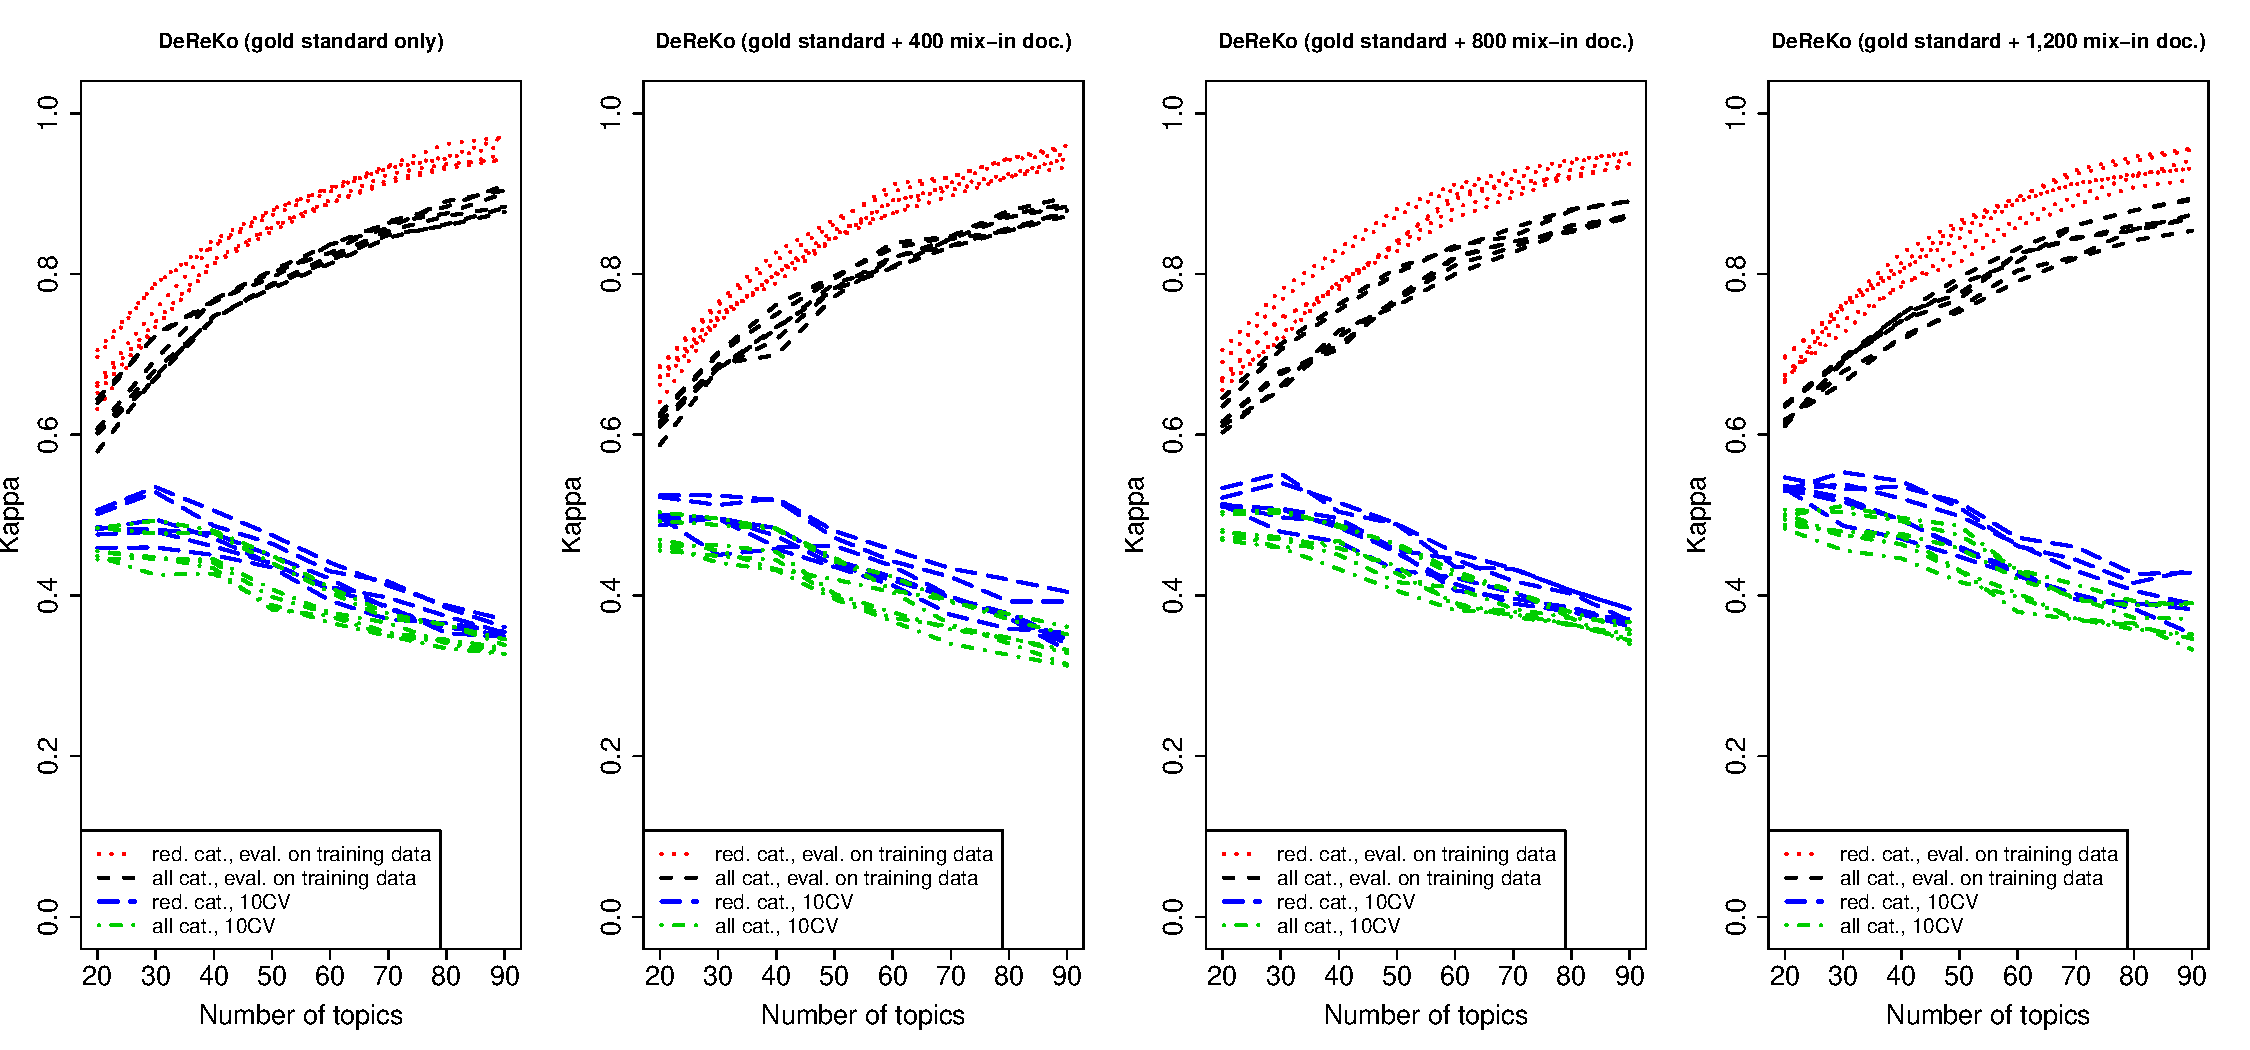
\includegraphics[width=\textwidth]{dereko_kappa}
%  \end{center}
%\end{frame}
%
%\begin{frame}
%  {Ergebnisse}
%  Zusammen ($\kappa$)\\
%
%  \begin{center}
%    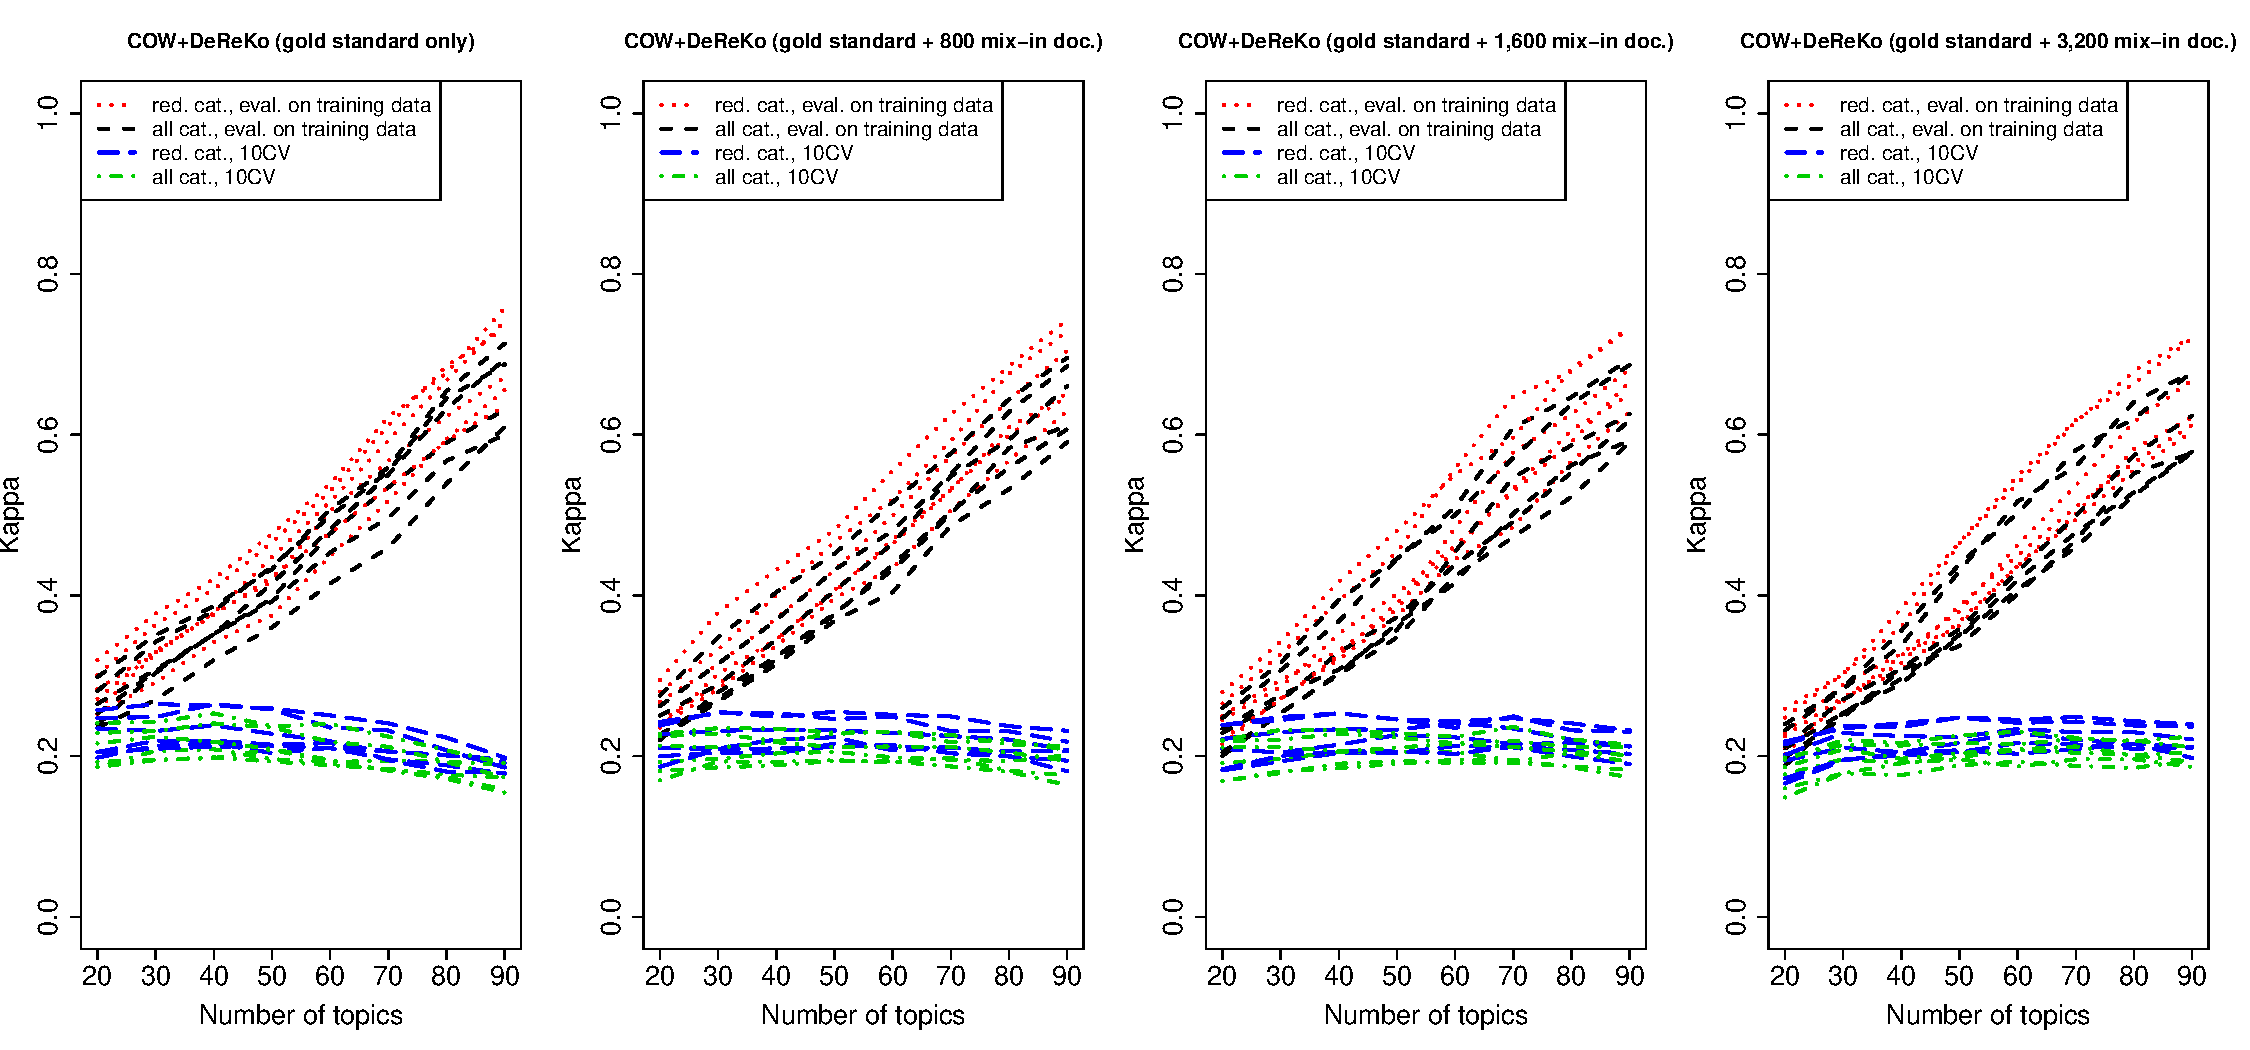
\includegraphics[width=\textwidth]{coreko_kappa}
%  \end{center}
%\end{frame}

\begin{frame}
  {Ergebnisse und Probleme}
  Evaluation\\

  \vspace{0.5cm}
  \resizebox{\textwidth}{!}{\begin{tabular}{lrrrr}
    \hline
    \textbf{Corpus} & \textbf{Accuracy} & \textbf{Precision} & \textbf{Recall} & \textbf{F-Measure} \\
    \hline
    COW &  \alert<2->{68.765\%} & 0.688 & 0.688 & 0.674 \\
    DeReKo & \alert<3->{72.999\%} & 0.725 & 0.730 & 0.696 \\
    COW + DeReKo & \onslide<4->{\alert{?}} & \onslide<4->{?} & \onslide<4->{?} & \onslide<4->{?} \\ 
    \hline
  \end{tabular}}
  \onslide<7->{~}
%  \vspace{0.5cm}
%  Diffusionsmatritzen\\
%
%  \vspace{0.5cm}
%  \resizebox{0.33\textwidth}{!}{\begin{tabular}{|llcccccccc|}
%    \hline
%    \multicolumn{2}{|c}{\textbf{COW}} & \multicolumn{8}{c|}{\textbf{Classified}} \\
%     && \rot{\textbf{PolSoc~}} & \rot{\textbf{Busi}} & \rot{\textbf{Life}} & \rot{\textbf{Arts}} & \rot{\textbf{Public~}} & \rot{\textbf{Law}} & \rot{\textbf{Beliefs~}} & \rot{\textbf{Hist}} \\
%   \hline
%   \multirow{8}{*}{\rot{\textbf{Annotated}}} & \textbf{PolSoc}  & \textbf{26} &  12 &  10 &   1 &   1 &   0 &   1 &   0 \\ 
%     & \textbf{Busi}    &  5 & \textbf{105} &  40 &   7 &   1 &   2 &   1 &   1 \\ 
%     & \textbf{Life}    &  3 &  14 & \textbf{286} &   6 &   4 &   1 &   1 &   1 \\ 
%     & \textbf{Arts}    &  3 &   2 &  36 &  \textbf{78} &   1 &   0 &   2 &   6 \\ 
%     & \textbf{Public}  &  0 &   3 &  11 &   0 &   \textbf{9} &   1 &   0 &   0 \\ 
%     & \textbf{Law}     &  3 &   9 &   8 &   0 &   1 &   \textbf{8} &   0 &   0 \\ 
%     & \textbf{Beliefs} &  4 &   3 &  11 &   6 &   1 &   0 &  \textbf{30} &   1 \\ 
%     & \textbf{Hist}    &  9 &   0 &   9 &   7 &   1 &   1 &   2 &  \textbf{15} \\ 
%     \hline
% \end{tabular}}~~\resizebox{0.25\textwidth}{!}{\begin{tabular}{|llcccccc|}
%    \hline
%     \multicolumn{2}{|c}{\textbf{DeReKo}} & \multicolumn{6}{c|}{\textbf{Classified}} \\
%     && \rot{\textbf{PolSoc~}} & \rot{\textbf{Busi}} & \rot{\textbf{Life}} & \rot{\textbf{Indiv}} & \rot{\textbf{Arts}} & \rot{\textbf{Public}} \\
%    \hline
%     \multirow{6}{*}{\rot{\textbf{Annotated}}}& \textbf{PolSoc}  & 223 & 6 & 39 &  0 &  0 &  8 \\
%     & \textbf{Busi}    &  20 & 24 &   9 &  0 &  0 &  0 \\
%     & \textbf{Life}    &  24 &  1 & 324 &  0 &  0 &  1 \\
%     & \textbf{Indiv}   &   5 &  0 &  17 &  0 &  0 &  1 \\
%     & \textbf{Arts}    &   2 &  0 &  28 &  0 &  6 &  0 \\
%     & \textbf{Public}  &  35 &  0 &  30 &  0 &  0 & 34 \\
%    \hline
% \end{tabular}}~~\resizebox{0.315\textwidth}{!}{\begin{tabular}{|llccccccccc|}
%    \hline
%     \multicolumn{2}{|c}{\textbf{Joint}} & \multicolumn{9}{c|}{\textbf{Classified}} \\
%     && \rot{\textbf{PolSoc~}} & \rot{\textbf{Busi}} & \rot{\textbf{Medical~}} & \rot{\textbf{Life}} & \rot{\textbf{Arts}} & \rot{\textbf{Public~}} & \rot{\textbf{Law}} & \rot{\textbf{Beliefs~}} & \rot{\textbf{Hist}} \\
%    \hline
%    \multirow{9}{*}{\rot{\textbf{Annotated}}} & \textbf{PolSoc}   & \textbf{199} &   7 &   0 & 109 &   0 &  12 &   0 &   0 &   0 \\ 
%    & \textbf{Busi}     &  18 &  \textbf{23} &   0 & 172 &   0 &   2 &   0 &   0 &   0 \\ 
%    & \textbf{Medical}  &   6 &   0 &   \textbf{0} &  29 &   0 &   1 &   0 &   0 &   0 \\ 
%    & \textbf{Life}     &  25 &   4 &   0 & \textbf{632} &   0 &   5 &   0 &   0 &   0 \\ 
%    & \textbf{Arts}     &   2 &   2 &   0 & 160 &   \textbf{0} &   0 &   0 &   0 &   0 \\ 
%    & \textbf{Public}   &  46 &   2 &   0 &  56 &   0 &  \textbf{19} &   0 &   0 &   0 \\ 
%    & \textbf{Law}      &   8 &   0 &   0 &  31 &   0 &   0 &   \textbf{0} &   0 &   0 \\ 
%    & \textbf{Beliefs}  &   0 &   0 &   0 &  59 &   0 &   0 &   0 &   \textbf{0} &   0 \\ 
%    & \textbf{Hist}     &   4 &   0 &   0 &  50 &   0 &   0 &   0 &   0 &   \textbf{0} \\ 
%    \hline
% \end{tabular}}

\end{frame}

%\begin{frame}
%  {Aktuell}
%  Was die Ergebnisse nahelegen\dots\\
%
%  \vspace{0.5cm}
%
%  \begin{itemize}
%    \item größere Goldstandards
%    \item Aufteilen überstark repräsentierter Kategorien
%    \item im Projekt \textit{linguistische Webcharakterisierung} (FU Berlin):\\
%      5000 Goldstandard-Dokumente angestrebt
%      \vspace{0.5cm}
%
%    \item<2-> Aber: \alert{Brauchen wir wirklich interpretierbare Kategorien?}
%  \end{itemize}
%\end{frame}

% --------------- REFS + APPENDIX

\begin{frame}[allowframebreaks]
  {References}
  \def\newblock{\hskip .11em plus .33em minus .07em}
  \footnotesize
%  \bibliographystyle{abbrvnat} 
  \bibliographystyle{natbib.fullname}
  \bibliography{coreko}
\end{frame}

\end{document}
